\documentclass[a4paper,twoside,12pt]{article}
\usepackage[T1]{fontenc}
\usepackage[utf8]{inputenc}
\usepackage[english]{babel}
\usepackage{enumerate}
\usepackage[shortlabels]{enumitem}
\usepackage{fullpage}
\usepackage{setspace}
\usepackage{graphicx}
\usepackage{import}
\usepackage{amsmath}
\usepackage{mathabx}
\usepackage{icomma}
\usepackage{booktabs}
\usepackage{ftcap}
\usepackage{lipsum}
\usepackage{url}
\usepackage[binary-units]{siunitx}
\usepackage{epstopdf}
\usepackage{hyperref}
\usepackage{subcaption}

\begin{document}
\thispagestyle{empty}
\begin{flushleft}
 \underline{Sakari} Matias Kapanen\hfill
 \texttt{sakari.m.kapanen@student.jyu.fi}
\end{flushleft}
\vfill
\begin{center}
\textsc{\LARGE A Monte Carlo code for simulating the neutral density profile in an ECR ion source}
\end{center}
\vfill
% Palautuspvm
Supervisor: Taneli Kalvas\\
\vfill
\begin{abstract}
 \noindent
    In this research training project work, a Monte Carlo code was developed in
    order to estimate the spatial distribution of neutrals in the vacuum
    chamber of an ECR ion source. The ECR plasma was treated as a stationary
    collection of ion and electron populations, allowing to effectively reduce
    the computational complexity of the simulation and not having to simulate
    individual plasma particles. Despite the approximations, qualitative
    results corresponding to experimental observations were seen. For example,
    accumulation of neutrals in the ion loss zones was observed.
\end{abstract}
\clearpage%

\setlength{\parindent}{0pt}
\setlength{\parskip}{12pt}

\setcounter{page}{1}

\section{Introduction}

In electron cyclotron resonance ion sources (ECRIS), it is crucial to keep the
neutral density low enough to achieve efficient production of high ion charge
states. The removal of neutrals is usually realized using turbo vacuum pumps.
There are usually vacuum gauges installed in some locations to monitor the pressure.

The gauges, however, cannot capture local deviations in the neutral density. Therefore, the problem was approached by means of numerical simulation. The goal of this research training project was to produce a Monte Carlo code which could be used for that purpose.

It was assumed that the flow of neutrals is in the molecular flow regime, i.e. there is no direct interaction between the neutrals. The groundwork for the free molecular flow simulation was laid earlier in the author's BSc thesis~\cite{kapanen:bsc}.

A self-consistent ECRIS Monte Carlo simulation code was recently developed by
Mi\-ro\-nov~\cite{mironov:ecr}. That code is based on the Particle-in-Cell method
and features a full dynamic model of the plasma ions and electrons. This kind
of a model typically leads
to great computational complexity, posing strong requirements on the choice of
simulation hardware.

In this project the idea of a simpler, quasi-stationary plasma model was probed. Such a model has the advantage of lower complexity because one only has mutually non-interacting neutrals as test particles. The independence of the test particles also means that the computation is easily parallelizable and performance gains can be had from running on multiprocessor systems.

The bulk of the work in this project consisted of implementing a suitable plasma model and implementing neutral ``ray tracing'' in a real CAD geometry.

\section{Theoretical background}
In a typical ECR ion source, a plasma is formed by injecting neutral gas particles into a vacuum chamber and coupling RF energy to it at the frequency of several $\si{\giga\hertz}$.

The plasma in an ECR ion source is a typical example of a laboratory plasma,
with an electron density of $\sim\SI{e11}{\per\centi\metre}$. Due to the
electron cyclotron resonance heating, there is a population of electrons with a
high average energy of several $\si{\kilo\electronvolt}$. However, there is
another population of electrons with lower energies. Thus, the electron energy
distribution isn't strictly Maxwellian.~\cite{geller:ecr}

Given that the ion confinement time in the magnetic bottle is long enough to achieve thermalization, the ion energy distribution can also be assumed as Maxwellian with a temperature of a few electronvolts~\cite{geller:ecr}.

\subsection{Plasma processes}
This section lists the collision processes where the plasma and neutrals are
involved. The focus is purposely kept on reactions concerning the neutrals. Also, only the ``single'' versions of these processes are covered as these dominate over the multiple counterparts in most cases. The formulae for the respective cross sections or rate coefficients are also listed.

Using the cross section $\sigma$, the rate coefficient is then defined as $\langle \sigma(v_r) v_r \rangle$ where $v_r$ is the speed of the target particle relative to the bombarding particles. Considering a population of bombarding particles whose velocities have a uniform direction distribution, the relative speed can be written as
\begin{equation}
    v_r = \sqrt{v_x^2 + v_y^2 + (v_z - v_t)^2}
\end{equation}
where $v_t$ is the speed of the target particle and $v_{\{x, y, z\}}$ are the velocity components of the bombarding particle. Here the direction of the target particle motion was chosen to be along the $z$ axis. This choice is arbitrary due to the symmetry of the velocity distribution of the projectile particles.

Now the rate coefficient can be calculated as an integral over the projectile particle velocity space:
\begin{equation}
    \label{eq:ratecoeff}
    \langle \sigma v_r \rangle = \int\limits_{-\infty}^\infty \int\limits_{-\infty}^\infty \int\limits_{-\infty}^\infty v_r \sigma(v_r) f(v_x, v_y, v_z)\,\mathrm{d}v_x\,\mathrm{d}v_y\,\mathrm{d}v_z,
\end{equation}
where $f(v_x, v_y, v_z)$ is the velocity distribution of the projectile particles. In the context of this simulation, $f$ is the Maxwellian velocity distribution:
\begin{equation}
    f(v_x, v_y, v_z) = \left(\frac{m}{2\pi kT}\right)^{3/2} \exp \left[ -\frac{m(v_x^2 + v_y^2 + v_z^2)}{2kT} \right]
\end{equation}
where $m$ is the projectile particle mass, $k$ is the Boltzmann constant and $T$ is the temperature of the projectile particle population.

\subsubsection{Electron ionization}
Electron (impact) ionization is a process where an energetic electron
positively ionizes a neutral by knocking off an electron bound to a shell:
\[
    X^0 + e \rightarrow A^{(n+1)+} + 2e,
\]
where $X$ is the neutral and $e$ is an electron. Electron ionization of already
positively charged ions is not considered here.

There have been many approximations of the electron ionization cross sections, most famously the Lotz equation~\cite{lotz}. A more convenient approximation was found in~\cite{recommended_ionization} and is given in the form of a fit function
\begin{equation}
    \label{eq:ionization_fit}
    \sigma(E) = \frac{1}{IE} \left[ A \ln \left(\frac{E}{I}\right) + \sum\limits_{i=1}^N
    B_i \left(1-\frac{I}{E}\right)^i \right]
\end{equation}
where $E$ is the electron energy, $I$ is the ionization potential of the atom
or ion and $A$, $B_i$ are fit parameters depending on the atom or ion. The fit
parameters are given in~\cite{recommended_ionization}. Notice that the cross
section is given as a function of the electron energy instead of the relative
speed --- however, because the electron speed is undoubtedly much greater than the target particle speed, this is a perfectly valid approximation.

For example, the fit parameters for argon neutrals are listed in table~\ref{table:argon_ionization}.
\begin{table}
    \centering
    \caption{Fit parameters of equation~\ref{eq:ionization_fit} for argon neutrals~\cite{recommended_ionization}.}
    \label{table:argon_ionization}
    \begin{tabular}{cccccccc}
        \toprule
        $I\,(\si{\electronvolt})$ & $A$ & $B_1$ & $B_2$ & $B_3$ & $B_4$ & $B_5$ & condition\\
        \midrule
        15.8 & 2.532 & -2.672 & 2.543 & -0.769 & 0.008 & 0.006 & \\
        15.8 & 4.337 & 3.092 & -21.253 & 14.626 & 0.018 & 0.031 & $E > 4.13I$ \\
        \bottomrule
    \end{tabular}
\end{table}

\subsubsection{Charge exchange}
Charge exchange is a process where an ion $X$ exchanges an electron with
another ion or a neutral $Y$:
\[
    X^{m+} + Y^{n+} \rightarrow X^{(m-1)+} + Y^{(n+1)+}.
\]
For example, $X$ being a $+1$ ion and $Y$ a neutral:
\[
    X^{1+} + Y^0 \rightarrow X^{0} + Y^{1+}.
\]

A famous approximation for the single charge exchange cross section is the one proposed by Salzborn et al. and used in~\cite{cex} as
\begin{equation}
    \label{eq:cex}
    \sigma_{q, q-1} = 1.43 \times 10^{-12} q^{1.17} I^{-2.76}\,(\si{\centi\metre\squared}),
\end{equation}
where $q$ is the initial charge of the projectile and $I$ is the ionization potential of the target particle in $\si{\electronvolt}$.

\subsubsection{Recombination}
In recombination, a free electron is bound onto a shell of an ion and the excess energy is released as a photon $\gamma$. If the release of energy happens ``directly'', the process is called radiative recombination:
\[
    X^{n+} + e \rightarrow X^{(n-1)+} + \gamma.
\]
The released energy can also excite another bound electron which then de-excites and emits a photon:
\[
    X^{n+} + e \rightarrow X^{(n-1)+**} \rightarrow X^{(n-1)+} + \gamma.
\]
This process is called dielectronic recombination.~\cite{nist:recombination}

Precalculated rate coefficients for these two processes at various different electron temperatures were found at~\cite{iaea:flychk}. The rate coefficients of the two processes were summed to yield a total recombination rate coefficient.

\subsection{Ion loss}
In addition to recombination, a remarkable neutralization channel is the loss
of ions from the magnetic bottle. When an ion is no longer confined by the
magnetic bottle, it eventually hits a wall of the vacuum chamber. Inelastic
collision reactions with the wall material eventually neutralize the ion and it
will be adsorbed.

\subsection{Knudsen's cosine law}
The desorption of neutrals from walls of the vacuum chamber is assumed to be governed by Knudsen's cosine law~\cite{knudsen:cosine}:
\begin{equation}
    \mathrm{d}n = \frac{n}{\pi}\cos\theta \,\mathrm{d}\omega,
\end{equation}
where $n$ is the flux of particles desorbing into the solid angle element $\mathrm{d}\omega$ and $\theta$ is the angle of $\mathrm{d}\omega$ with respect to the surface normal.

\subsection{Thermal accommodation}
When a particle is adsorbed onto a wall, it may be only partially thermalized with the wall before desorption. The efficiency of this thermalization process is characterized by the \emph{accommodation coefficient} $\alpha$, which depends on the surface material, surface finish and the element of the incoming particles. It is defined according to the equation
\begin{equation}
    \alpha = \frac{E_\text{in} - E_\text{re}}{E_\text{in} - E_\text{w}},
\end{equation}
where $E_\text{in}$ is the incoming energy flux, $E_\text{re}$ the reflected flux and $E_\text{w}$ the emitted energy flux in the case of full thermalization.~\cite{sandia:accom}

\section{Numerical methods and tools}
Several numerical methods and software packages were used to implement the
calculation of the neutral density distribution. The actual implementation code
can be found in a Git repository~\cite{kapanen:git}.

\subsection{Monte Carlo test particle simulation}
The basis of the simulation is the test particle Monte Carlo method. A limited set of test particles is chosen to represent the real particles and given a corresponding statistical weight in the simulation. Their phase space coordinates are randomly drawn from the corresponding probability distributions and propagated through the target geometry. On wall collisions, a new direction and velocity are calculated according to Knudsen's cosine law and the thermal accommodation law. The test particle simulation of neutrals without plasma is covered in detail in~\cite{kapanen:bsc}.

\subsection{A simple quasi-stationary plasma model}
The plasma model implemented in this simulation describes the plasma electrons and ions of different charge states as density distributions defined in a cubic grid. The velocities of the plasma particles are approximated as Maxwellian with predefined temperatures.

Taking the conservation of the plasma mass as a guiding principle, the following approximations were made:
\begin{itemize}
    \item Stationarity: the plasma population parameters (density, temperature) are not affected by collision reactions.
    \item The spatial density distributions of the ion populations are
        proportional to the distribution of electrons. The code takes the
        global charge state distribution as an input.
    \item The plasma consists of only one element.
    \item Elastic collisions between the neutrals and the plasma particles are neglected.
\end{itemize}

An ionizing collision reaction may result in excess mass accumulating in the plasma. Conservation of mass is implemented here: the plasma must eventually emit a particle through some channel.

In this simulation, the two collision processes involving neutrals are charge exchange and electron ionization. In charge exchange, the plasma mass offset is unchanged because an ion is neutralized but the plasma also receives a new ion. Thus there is no need to emit an additional neutral. In electron ionization, a neutral comes in and is ionized by an electron, thus the plasma gains an excess of one particle. The excess is compensated by statistically choosing a neutralization channel and the corresponding neutralization time.

\subsubsection{Monte Carlo collisions}
To handle collisions processes of neutrals with the plasma particles (ions and electrons), a Monte Carlo collision method has to be used. The electrons and ions don't exist in the simulation as individual test particles but as particle distributions.

Consider a test particle traveling through a particle population bombarding it at the frequency $\nu$. Remembering that a single test particle represents multiple real particles, the propagation of the test particle can be seen as probability flux or an ``intensity''. The calculation of collision probabilities arises from the differential equation
\begin{equation}
    \frac{\mathrm{d}p}{\mathrm{d}t} = -\nu p(t),
\end{equation}
where $p$ is the particle probability flux and $t$ the time. Setting $p(0) = 1$, The solution to this differential equation is
\[
    p(t) = \exp(-\nu t).
\]
The collision probability is now found as the complement:
\begin{equation}
    p_\text{coll} = 1 - \exp(-\nu t),
\end{equation}
where $\nu$ is the rate of the collision reaction in question. Considering a test particle propagating by a timestep $\Delta t$ in a projectile particle cloud of density $n_i$ and the rate coefficient of the reaction is $\langle v_r \sigma_i \rangle$, the probability of the collision happening during the timestep is
\begin{equation}
    p_i = 1 - \exp(-n_i \langle v_{r, i} \sigma_i \rangle \Delta t),
\end{equation}
where $v_{r, i}$ is the relative speed of the test particle to the projectile population. Drawing a pseudo-random number $x \in [0, 1[$, a collision now happens if
\[
    x \leq p_i = 1 - \exp(-n_i \langle v_{r, i} \sigma_i \rangle \Delta t),
\]
or equivalently
\[
    x > \exp(-n_i \langle v_{r, i} \sigma_i \rangle \Delta t).
\]

When there are multiple populations and collision reactions, the total collision frequency is calculated as:
\begin{equation}
    \nu_\text{tot} (v) = \sum\limits_i \nu_i = \sum\limits_i n_i \langle v_{r, i} \sigma_i \rangle,
\end{equation}
where $i$ runs over different collision reactions.
In practice, the values $\langle v_{r, i} \sigma_i \rangle$ are expensive to calculate and are thus precomputed in a grid of some fixed values of $v$ and stored in an array. Linear interpolation between the gridpoints is used to acquire the collision frequency at arbitrary values of $v$.

The total collision frequency is used at each timestep to decide if a collision has happened. In the case of a collision, the collision reaction type $i$ is randomly decided using the individual reaction rates as the probability distribution:
\begin{equation}
    p[i] = \frac{\nu_i}{\nu_\text{tot}}.
\end{equation}
Given a pseudo-random number $x \in [0, 1[$, the chosen reaction is the smallest value of $i$ such that
\[
    x \leq \frac{\sum\limits_{j=0}^i \nu_j}{\nu_\text{tot}}.
\]

When the decision on the collision process is made, a projectile particle is sampled from the corresponding particle population. The collision dynamics are then calculated in the center-of-mass frame. The neutral product (if any) is then tracked further.

The reactions handled in the way described above in the simulation are charge exchange and electron ionization.

\subsubsection{Neutralization channel sampling}
If the plasma mass offset is increased due to an ionizing reaction, a particle will be emitted from the plasma and eventually neutralized. There is the possibility of specifying one or more neutralization channels, each of which follows an exponential decay law:
\begin{equation}
    p_\text{neutralized}(t) = 1 - \exp(-t / \tau_i ),
\end{equation}
where $p_\text{neutralized}$ is the probability that the neutralization
reaction has happened withing time $t$ and $\tau_i$ is the time constant of the corresponding reaction. Given a pseudo-random number $x \in [0, 1[$, a random neutralization time can be sampled by conventional inverse transform sampling:
\begin{equation}
    t = -\tau_i \ln x.
\end{equation}

Because the neutralization neutralization processes are independent from each other, the following way of sampling is implemented:
\begin{enumerate}
    \item For each neutralization channel, sample a random decay time.
    \item Choose the reaction with the shortest decay time.
\end{enumerate}

Practically, recombination and loss of an ion from magnetic confinement are the two neutralization processes. In recombination, the position of the reaction is sampled from the 1+ ion density distribution. The velocity of the resulting neutral is sampled according to the 1+ energy distribution (Maxwell).

The magnetic loss is a bit more complicated. Predefined ``loss zones''
calculated in an electron simulation are used. These are regions on the walls
of the chamber where lost electrons have hit. The spatial behaviour of a plasma
is usually dominated by the electrons and thus the ion loss zones should
roughly correspond to the electron loss zones as seen in~\cite{kalvas:hiisi}. When an ion escapes through this channel, its position on the wall is chosen randomly according to the loss zones and it is assumed to be fully thermalized with the wall and neutralized due to recombination with wall electrons. Then a neutral is emitted from this position according to the cosine law.

\subsection{Electron simulation}
A simple, single electron simulation was used to calculate the electron distribution of the plasma. The electrons are simulated individually. Their trajectories are simulated in the target geometry which is approximated by a cylinder in the presence of a magnetic field. The magnetic field is given by the superposition of an axisymmetric expansion of the solenoid field and an ideal hexapole field. The single electron model is described in detail in~\cite{kalvas:hiisi}.

The points where the electrons hit the chamber walls were recorded. Also, at each timestep, the locations of the electrons were recorded by incrementing the corresponding counters in a cube grid. From this grid of counters, the electron density was calculated by normalization. The choice of normalization is not exact. In the chosen approach, cells with counter value of 1/4 or more of the global maximum value were regarded as plasma cells. The normalization factor was chosen such that the average density in these cells evaluated to unity.

The coordinates of the electron endpoints corresponding to the ``loss zones'' mentioned earlier and the electron density distribution were stored as CSV data files.

\subsection{Calculating the confinement time}
\label{sec:confinement}
Lastly, the confinement time of ions in the magnetic bottle had to be estimated. Geller~\cite{geller:ecr} gives an equation for ions of charge state $q+$:
\begin{equation}
    \label{eq:confinement_time}
    I_q \simeq \frac{1}{2} \frac{n_q q e \mathrm{Vol}}{\tau_q},
\end{equation}
where $I_q$ is the extracted ion current, $n_q$ is the ion density, $e$ is the elementary charge, $\tau_q$ the confinement time and Vol is the volume bounded by the magnetic field lines which lead to the extraction hole.

This equation can be solved for $\tau_q$ using measured extraction current. However, the volume Vol had to be estimated. A simple Monte Carlo approach was used here: $N$ random positions were uniformly sampled on the extraction hole. The magnetic field lines starting from these points were traced backwards until the chamber wall was intersected, flagging the cells of a cube grid through which the field line passed. The volume Vol was the calculated as the sum of the volumes of these cells.

The magnetic field line backward tracing is implemented by numerically solving the differential equation
\begin{equation}
    \frac{\mathrm{d}\mathbf{s}(t)}{\mathrm{d}t} = -\mathbf{B}(\mathbf{s}(t)),
\end{equation}
where $\mathbf{s}(t)$ is the field line parametrized by the parameter $t$ and $\mathbf{B}$ is the total magnetic flux density.

\subsection{Software design}
One of the major challenges in the software design was efficiently calculating intersections of neutral paths with a CAD geometry with a non-trivial number of vertices and faces (given as STL files). The Computational Geometry Algorithms Library (\textsc{CGAL})~\cite{cgal} was chosen as the provider of algorithms related to manipulation of triangulated meshes. This choice implied the usage of \textsc{C++} as the programming language, which also made sense in terms of performance optimization.

The GNU Scientific Library (\textsc{GSL})~\cite{gsl} was used for the computation of the rate coefficient integrals~\eqref{eq:ratecoeff} and tracing the magnetic field lines as described in section~\ref{sec:confinement}.

The software library was designed with extensibility in mind. There are programming interfaces for moderately easy addition of new collision reactions and neutralization channels. Features of the modern \textsc{C++14} standard such as smart pointers were used for safe handling of memory. This is a subject that could still be improved upon, especially regarding read and write access of the \texttt{std::vector}s storing the density distribution.

The neutrals were tracked individually one by one, sampling the particle position and incrementing the respective counter in a cube grid at fixed intervals. The implementation uses multiple threads allowing many neutrals to be traced simultaneously and increasing performance on multicore systems.

The output data was stored as CSV files for postprocessing and plotting.

\section{Results}
Time-dependent and stationary simulations were run to test the simulation code. A simplified solid CAD model of the upcoming JYFL ECRIS HIISI was produced using OpenSCAD~\cite{openscad} and used as the target geometry. Originally an STL exported from the full CAD model was tried. However, the intersection calculation was found to be too expensive probably due to spatially imbalanced distribution and the great number of primitives.

\subsection{Simulation parameters}
Because as of writing this report there are no measurement of HIISI plasma parameters, some parameters from the JYFL 14 GHz ECRIS~\cite{jyfl:ecris14} were used. In particular, measured values of the extraction ion current of different charge states were used to obtain the charge state distribution. Additionally, the extraction current of 8+ ions was used to calculate the confinement time $\tau_{8+}$ from equation~\eqref{eq:confinement_time}. This confinement time was used as an approximation for all charge states. The calculation yielded a value of $\tau \approx \SI{1.9}{\milli\second}$.

The average electron density was assumed to be $\SI{e11}{\per\centi\meter\cubed}$. The electron energy distribution was taken to be Maxwellian, $T = \SI{10}{\kilo\electronvolt}$. This approximation neglects the cold electron distribution.

The element chosen for the gas feed was argon. Gas was fed to the chamber from the injection tube. The injection and extraction holes were configured as pumps with pumping efficiencies of 1 and 0.1, respectively.

\subsection{Stationary density distribution}
A stationary density distribution was calculated using the argon feed rate of
$\SI{1}{\centi\metre\cubed\per\hour}$ in NTP conditions which is a typical
value~\cite{tarvainen:phd}. Ten million test particles were used. Slices of the neutral density distribution on different axes were plotted.

One of the main observations from the plots is the accumulation of neutrals near the loss zones in the grooves of the vacuum chamber and the injection and extraction ends. This corresponds to the loss of ions from the magnetic confinement and neutralization on the wall. The accumulation can be seen in figures~\ref{fig:stationary_x} and~\ref{fig:stationary_z}.

\begin{figure}
    \centering
    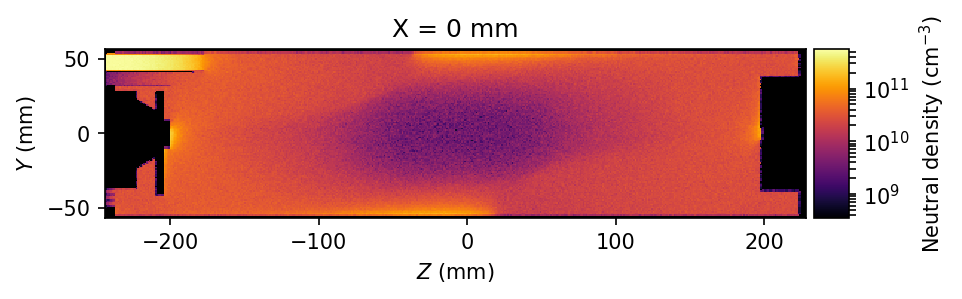
\includegraphics[width=\textwidth]{images/stationary_x_middle.png}
    \caption{A slice of the stationary neutral density distribution in the
    middle of the $X$ axis. The injection end is on the left, extraction end is
    on the right. Accumulation of neutrals can be seen on both ends and the
    cylinder walls in the middle.}
    \label{fig:stationary_x}
\end{figure}

\begin{figure}[t]
    \centering
    \begin{subfigure}{0.5\textwidth}
        \centering
        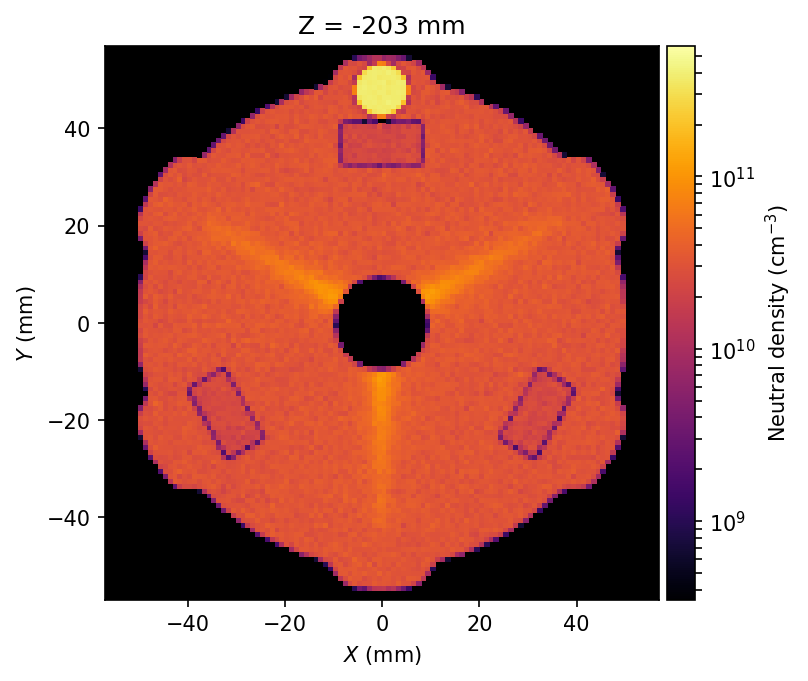
\includegraphics[width=\linewidth]{images/stationary_injection_end.png}
    \end{subfigure}%
    \begin{subfigure}{0.5\textwidth}
        \centering
        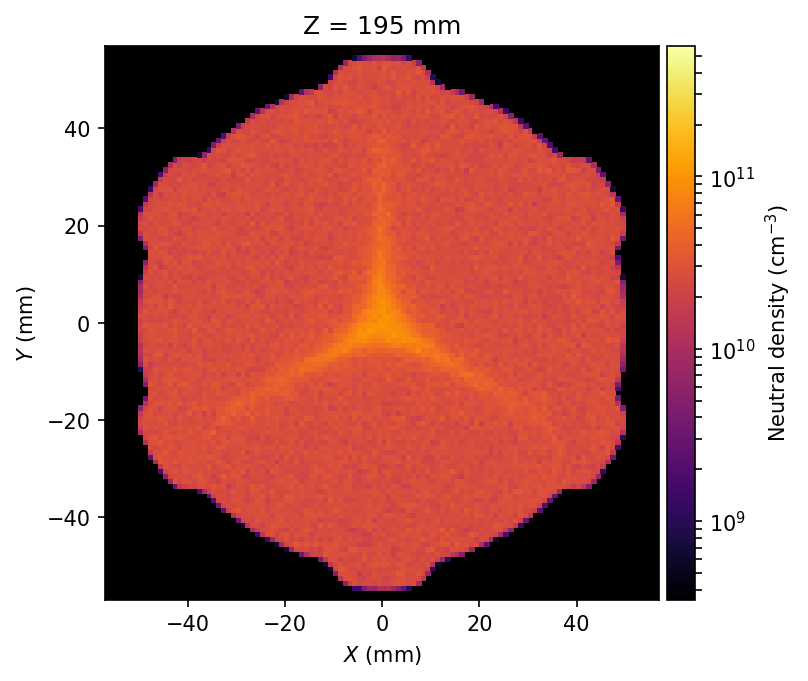
\includegraphics[width=\linewidth]{images/stationary_extraction_end.png}
    \end{subfigure}
    \begin{subfigure}{0.5\textwidth}
        \centering
        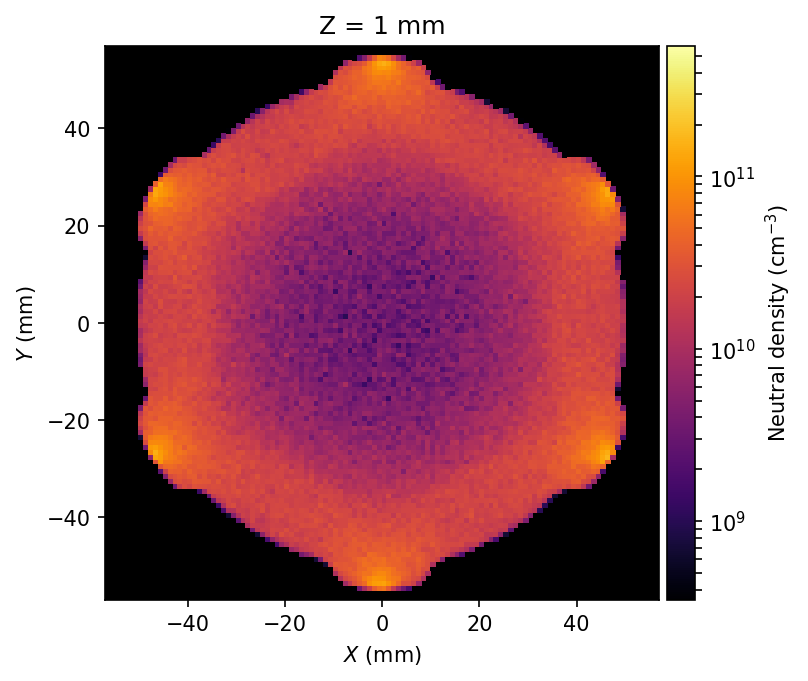
\includegraphics[width=\linewidth]{images/stationary_z_middle.png}
    \end{subfigure}
    \caption{Slices of the stationary neutral density distribution along the
    $Z$ axis at the injection end, extraction end and the middle of the
    chamber, showing the accumulation zones of the neutrals.}
    \label{fig:stationary_z}
\end{figure}

The neutral density in the middle of the chamber (in the plasma region) seems to be at least an order of magnitude lower than the surrounding one, below $\SI{e10}{\per\centi\metre\cubed}$. This is due to the internal pumping effect caused mainly by the electron ionization process. The internal pumping makes it possible to meet the criterion for multiply charged ion production, $n_e / n_0 \gg 1$.

From the reaction statistics, it is additionally seen that only a negligible number of the neutralizations happen through recombination.

\subsection{Convergence test}
To observe the convergence of the stationary neutral density distribution, the calculation was performed with several different numbers of test particles. The largest number was $N = 10^{7}$ and this result was taken as the ``correct'' distribution. The global error of the distributions obtained with lower number of statistics was then calculated using the $\ell^2$ norm:
\begin{equation}
    \delta = \sqrt{\sum\limits_{i \in \text{grid cells}} (n_i - \hat{n}_i)^2},
\end{equation}
where $\hat{n}_i$ is the neutral density in cell $i$ in the reference distribution ($N = 10^{7}$) and $n_i$ is the neutral density in the distribution whose error is being calculated.

The resulting data points and a line fit in $(\log N, \log \delta)$ coordinates are shown in figure~\ref{fig:convergence}. The slope of the fitted line is $-0.44 \pm 0.03$ and tells that the power law governing the convergence rate is
\[
    \delta \propto N^{-0.44},
\]
which coincides well with the known result that the convergence rate of a Monte Carlo integration method should be~\cite{kapanen:bsc}
\[
    \delta \propto \frac{1}{\sqrt{N}}.
\]

\begin{figure}[t]
    \centering
    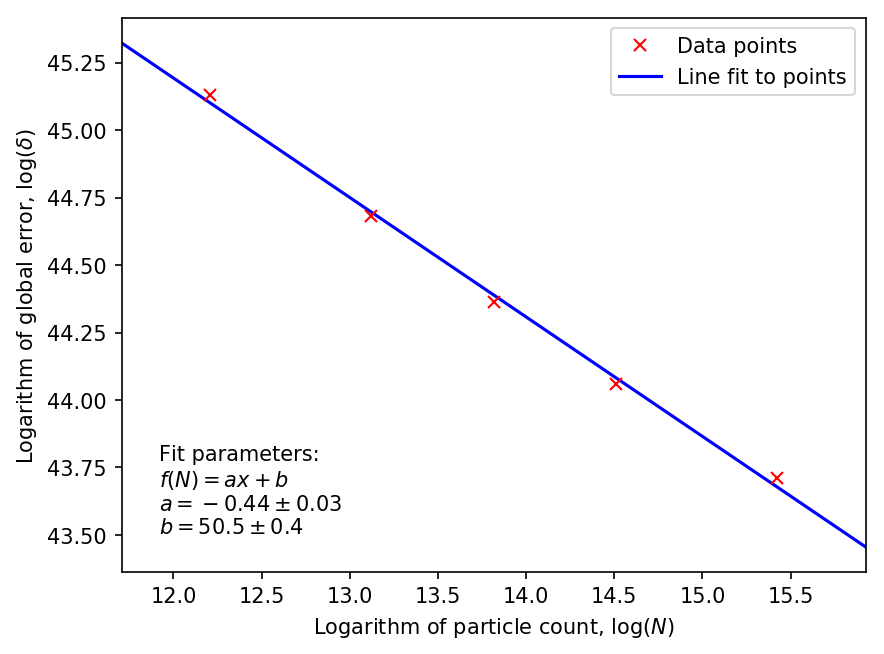
\includegraphics{images/convergence_plot.png}
    \caption{Global error plotted as the function of total test particle
    number and a line fit to the data points. In the $\log-\log$ coordinates,
    the slope of the line equals to the convergence power law.}
    \label{fig:convergence}
\end{figure}

The power law is not exactly $-0.5$ but pretty close --- this is due to the probabilistic nature of the Monte Carlo simulation. Therefore the convergence rate can be regarded as sensible.

\subsection{Time dependent density distribution}

Finally, a time dependent simulation with the same geometry and plasma
parameters as the stationary one. A gas pulse lasting $\SI{1}{\milli\second}$
consisting of $3 \times 10^{12}$ physical particles was injected into the
geometry via the injection tube, corresponding to some typical parameters used
in a particular light diagnostic setup~\cite{kronholm:ecr} developed at JYFL. $10^8$ simulation particles were used
for the simulation. The propagation of the gas pulse was tracked for
$\SI{10}{\milli\second}$ and sampled at $\SI{2}{\milli\second}$ intervals. Some
frames are plotted in figure~\ref{fig:time_dependent}.

\begin{figure}
    \centering
    \begin{subfigure}{0.8\textwidth}
        \centering
        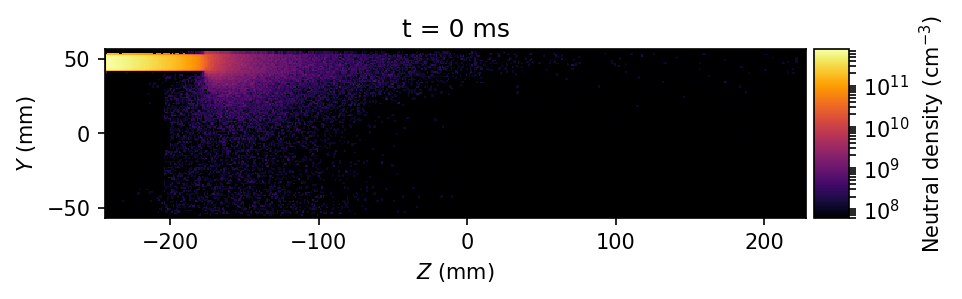
\includegraphics[width=\linewidth]{images/time_slice_00.png}
    \end{subfigure}
    \begin{subfigure}{0.8\textwidth}
        \centering
        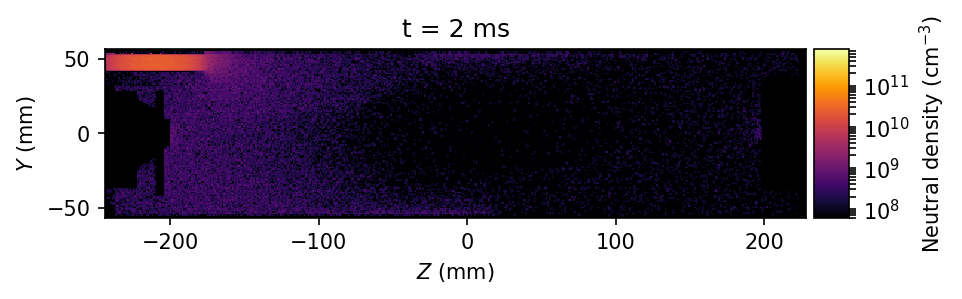
\includegraphics[width=\linewidth]{images/time_slice_02.png}
    \end{subfigure}
    \begin{subfigure}{0.8\textwidth}
        \centering
        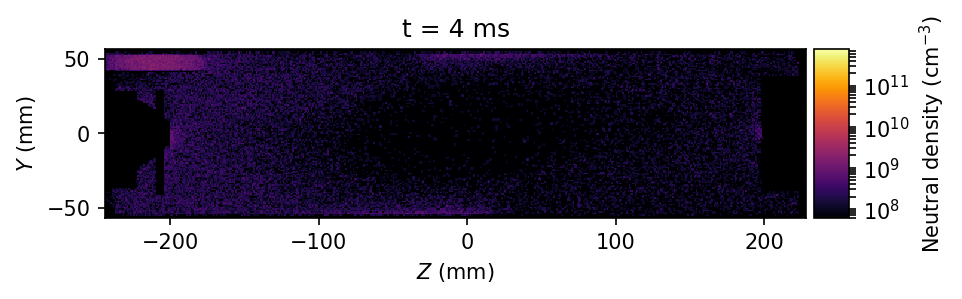
\includegraphics[width=\linewidth]{images/time_slice_04.png}
    \end{subfigure}
    \begin{subfigure}{0.8\textwidth}
        \centering
        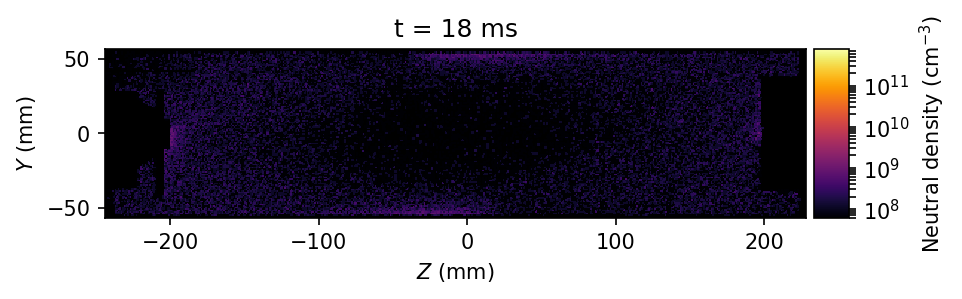
\includegraphics[width=\linewidth]{images/time_slice_18.png}
    \end{subfigure}
    \caption{Results of the time dependent simulation.}
    \label{fig:time_dependent}
\end{figure}

The main observation from the time series is how the gas pulse is quickly
diffused by the plasma reactions and wall collisions. The neutral density
distribution then seems to settle and the neutrals are accumulated in the loss
zones. These results coincide well with the quick rise and the slow decay of
the light signal in~\cite{kronholm:ecr}. If the simulation was continued
further, all the particles would eventually be removed from the system through
pumping channels.

\section{Conclusions}

There were many approximations made when implementing the plasma model.
In particular, neglecting the cold electron population is a significant
approximation and may have caused the negligible presence of
recombination reactions compared to other plasma processes.

It has been also observed in real ECR ion sources that the gas injection
remarkably affects the plasma parameters. Thus the stationary plasma model used
in this simulation may not hold valid especially in time-dependent simulations.
In the stationary simulations the use of such a model is more justifiable, at
least if the plasma parameters are measured in similar conditions (continuous
gas feed).

Many simulation parameters such as the extraction efficiency coefficient and
accommodation coefficient were left to be guessed. Therefore one must not
interpret the simulation results too strictly --- they are best taken as
qualitative, order-of-magnitude descriptions of the distribution of neutrals in
the vacuum chamber.

Comparing to a full-blown PIC model like Mironov's~\cite{mironov:ecr}, one
disadvantage of this code besides the approximations mentioned above is the
need for many input parameters like the charge state distribution. This is due
to the fact that this code is not self-consistent. On the other hand, the model
proposed in this research project is computationally less complex than a PIC model
and run times are most certainly shorter.

Despite the approximations, the code managed to capture some interesting
phenomena. First, the bombardment of ions on the loss zones seen
in~\cite{kalvas:hiisi} is related to the localization of neutrals in the same
zones in this simulation. Second, the quick rise and slow decay of the light
signal waveform obtained in~\cite{kronholm:ecr} corresponds to the time
dependent results from the simulation.

Another strength of this simulation method is the scalability to multiprocessor
systems. At least with the used HIISI geometry, the simulations could be run
with sufficient statistics with reasonable durations, lasting 1-2 days per
simulation run on a multicore laptop processor.

Due to the fact that the individual test particle histories are independent of
each other in this model, the model can be considered linear: the net effect of
several neutral sources can be found as the linear combination of the
individual neutral density profiles. This means that, for example, the
background neutral
distribution caused by outgassing and leakage (see~\cite{kapanen:bsc} for some
estimates) could be
precomputed and combined with a profile caused by gas injection to acquire the
total distribution. This makes it possible to obtain an overall, qualitative
picture of the relationships between the neutral densities in various locations in the
geometry. This information could be used to deduce and estimate the internal
neutral density based on readings of the vacuum gauges located at injection and
extraction.

Developing a multiprocessor physics simulation code that handles
large amounts of memory in \textsc{C++} is not the easiest task one could tackle
in a research training project. Not being in the know of various
memory safety features introduced in the modern \textsc{C++11} and
\textsc{C++14} standards beforehand, the author had to about learn these the hard way.
After many fruitful debugging sessions and refactoring to embrace safer
coding practices, the code works well and should be extensible with
new processes quite easily.

\clearpage

\bibliographystyle{unsrt}
\bibliography{references}

\end{document}

